\documentclass[a4paper,times,12pt]{article}
\usepackage{amsthm}
\usepackage[figuresright]{rotating}
\usepackage{graphicx}
\usepackage{booktabs}
\graphicspath{ {./images/} }
\usepackage{amssymb}
\usepackage{graphicx}
\usepackage{fancybox}
\usepackage{amsmath}
\usepackage{picinpar}
\usepackage{colortbl}
\usepackage{wasysym}
\usepackage{txfonts}
\usepackage{pb-diagram}
\usepackage{relsize}
\usepackage{tikz}
\usepackage{pgfplots}
\usepackage{subfigure}
\usepackage{algorithm}
\usepackage{algorithmic}
\usepackage{geometry}

\geometry{
  a4paper,        
  left=2.5cm,     
  right=2.5cm,    
  top=2.5cm,      
  bottom=2.5cm    
}

\begin{document}
\title{ANÁLISE DE DIFERENTES ALGORITMOS DE APRENDIZADO DE MÁQUINA PARA RECOMENDAÇÃO DE RESULTADOS NA FRANQUIA COUNTER STRIKE}
\begin{titlepage}
  \begin{center}

    %\begin{figure}[!ht]
    %\centering
    %\includegraphics[width=2cm]{c:/ufba.jpg}
    %\end{figure}

    \Huge{Instituto de Bioci\^{e}ncias, Letras e Ci\^{e}ncias Exatas, Unesp}\\
    \large{Departamento de Ciência da Computação e Estatística}\\ 

    \vspace{15pt}
    \vspace{95pt}
    {\LARGE{ANÁLISE DE DIFERENTES ALGORITMOS DE APRENDIZADO DE MÁQUINA PARA RECOMENDAÇÃO DE RESULTADOS NA FRANQUIA COUNTER STRIKE}} \\
    \title{{\large{Título}}}
    \vspace{3,5cm}
    Carlos Eduardo Nogueiro Silva\\
    Felipe Gomes da Silva \\
    Felipe Matheus Possari \\
    Renan Sinhorini Pimentel \\
  \end{center}


  \vspace{1cm}
  \begin{center}
    \vspace{\fill}
    Novembro\\
    2024
  \end{center}
\end{titlepage}
%%%%%%%%%%%%%%%%%%%%%%%%%%%%%%%%%%%%%%%%%%%%%%%%%%%%%%%%%%%%%%%%%%%%%%%%%%%%%
%%%%%%%%%%%%%%%%%%%%%%%%%%%%%%%%%%%%%%%%%%%%%%%%%%%%%%%%%%%%%%%%%%%%%%%%%%%%%
\newpage
\tableofcontents
\thispagestyle{empty}
\newpage

%%%%%%%%%%%%%%%%%%%%%%%%%%%%%%%%%%%%%%%%%%%%%%%%%%%%%%%%%%%%%%%%%%%%%%%%%%%%%
%%%%%%%%%%%%%%%%%%%%%%%%%%%%%%%%%%%%%%%%%%%%%%%%%%%%%%%%%%%%%%%%%%%%%%%%%%%%%

\section{Introdução}
\hspace{+15pt} 
Durante anos, os e-sports, apesar de atuarem no âmbito eletrônico, não utilizaram amplamente as estatísticas e dados de jogos para embasar as decisões táticas e/ou não esportivas. Porém, recentemente, esses dados foram fortemente inseridos no cenário competitivo profissional, especialmente na franquia Counter-Strike, que é o nosso objeto de estudo.

O volume de dados gerado nas grandes competições promove, de forma quase intuitiva, a necessidade de estabelecermos modelos precisos que analisem o desempenho de grandes nomes do cenário. Assim, podemos interpretá-los em diferentes âmbitos, seja para avaliações técnicas e táticas ou para resultados esportivos, gerando ao usuário do modelo uma menor incerteza sobre resultados que transitam entre o acaso do esporte e a precisão das estatísticas.

\section{Objetivos}
\hspace{+15pt}
Neste projeto, abordaremos a problemática de como diferentes algoritmos de aprendizado de máquina se comportam quando treinados com dados de Counter Strike, utilizando um sistema de rating. O objetivo principal é determinar a probabilidade de vitória de ambos os times, uma vez que essa informação pode ser útil para inúmeros casos, assim como em apostas esportivas.


\section{Justificativa}
\hspace{+15pt}
A escolha do tema foi pensada para oferecer uma vantagem significativa em termos de estratégia, seja para os próprios times, analistas ou até mesmo para o público que acompanha o cenário competitivo e realiza apostas. A estatística desempenha um papel fundamental neste estudo, pois possibilita a modelagem da incerteza e a análise de tendências com base em dados concretos.

De acordo com o estudo de Ondřej Švec (2022), um modelo baseado em ELO seria a melhor escolha para a predição de resultados, podendo alcançar até 64\% de acurácia. Faz-se necessário, então, unir dados reais e avaliações anteriores, como o ELO, em busca de uma recomendação precisa de resultados.

\section{5W1H}
\subsection*{What – O que vamos fazer?}
\hspace{+15pt}
Faremos um estudo da base de dados do Kaggle:\cite{Kaggle}, que contém mais de três mil partidas profissionais de Counter Strike. 
Utilizando estes dados escolheremos um modelo de classificação baseado em aprendizado de máquina para a análise dos dados. Uma vez feita essa escolha, usaremos esse modelo para gerar predições de resultados de partidas de Counter Strike.

\subsection*{Where – Para onde estamos olhando?}
\hspace{+15pt}
Utilizaremos dados de times do mais alto nível de competição do jogo, os 30 melhores times, ranqueados pelo site hltv.org, uma plataforma muito conhecida no meio competitivo de CSGO, dos maiores campeonatos dos anos em questão. 
O estudo terá ênfase nas estatísticas gerais do time, usando parcilamente dados individuais de cada jogador, uma vez que esses dados não refletem corretamente o desempenho da equipe como um todo.

\subsection*{When – Para quando estamos olhando?}
\hspace{+15pt}
A base escolhida possui dados de partidas jogadas em grandes campeonatos entre os anos 2016 e 2020, portanto o estudo busca prever os resultados das partidas dos anos posteriores a 2020.

\subsection*{Who – Para quem é este estudo?}
\hspace{+15pt}
O público alvo desse estudo são usuários de plataformas de aposta, em específico as que possuem a categoria Counter Strike, uma vez que com os resultados que buscamos, será possível prever ganhadores de futuras partidas. Dessa forma esperamos poder guiar os apostadores a maiores lucros.
Mesmo não sendo o público alvo principal, também buscamos auxiliar jogadores de times profissionais e suas respectivas comissões técnicas, uma vez que não analisaremos apenas resultados e sim dados gerais dos times.

\subsection*{Why – Por que estamos fazendo este estudo?}
\hspace{+15pt}
O motivo da escolha do tópico se dá não só pela afinidade que possuímos com o jogo, mas principalmente da escassez de estudos estatísticos e probabilísticos aprofundados nessa área. 
Com o aumento da popularidade não somente do jogo mas também das plataformas de aposta, possuímos um grande incentivo e um público cada vez maior capaz de usufruir dos resultados e análises do nosso estudo.

\subsection*{How - Como vamos fazer?}
\hspace{+15pt}
Primeiramente faremos o pré-processamento dos dados para filtrar apenas os dados que realmente importam para a análise.

Após isso, utilizaremos um sistema Elo para cada um dos times com base em fórmulas estabelecidas por Arpard Elo, inicialmente criadas para classificar jogadores de xadrez.
Realizando alguns ajustes nas aplicações das fórmulas, usaremos um modelo de classificação com aprendizado de máquina para realizar as predições por meio do treinamento do modelo com os dados que possuímos.


\section{Fonte de Dados}
\hspace{+15pt}
Inicialmente, tentou-se coletar dados através de \textbf{web scraping} de sites especializados, como o \textbf{HLTV}, que fornece estatísticas detalhadas de partidas profissionais. No entanto, devido a restrições impostas pelo site (banimento por IP) por muitas requisições ao servidor, foi necessário alterar a estratégia de coleta. Optou-se, então, por utilizar o "CS* Professional Matches Dataset" disponível no Kaggle  disponível em: \cite{Kaggle}, que oferece um conjunto abrangente de dados das partidas entre os principais times profissionais.
\subsection{Descrição do Dataset}
\begin{itemize}
  \item \textbf{Período Coberto:} 2016 a 2020.
  \item \textbf{Times:} Partidas envolvendo os times presentes no top 20 do ranking global durante o período.
  \item \textbf{Estatísticas Individuais:} Dados como \textbf{rating}, \textbf{impacto}, \textbf{taxa de kills por morte (KDR)}, \textbf{dano médio por round (DMR)}, \textbf{kills por round (KPR)}, \textbf{assistências por round (APR)}, entre outros.
  \item \textbf{Informações dos Times:} Inclui o \textbf{ranking mundial}, \textbf{porcentagem de vitórias em confrontos diretos (head-to-head)}, \textbf{Elo}, entre outros.
\end{itemize}
\section{Pré-processamento dos dados}
\hspace{+15pt}
Foram removidas do dataset todas as informações que só estariam disponíveis após o término das partidas, como os \textbf{pontos finais de cada time} e o \textbf{resultado da partida}. Isso evita a introdução de viés e garante que o modelo utilize apenas informações que estariam disponíveis antes do início de uma partida real.
\subsection{Cálculo do Elo dos Times}

\hspace{+15pt}
O sistema Elo, originalmente desenvolvido por Arpad Elo para ranquear jogadores de xadrez, foi adaptado para diversas competições e esportes ao longo dos anos, incluindo o cenário competitivo de \textbf{Counter-Strike: Global Offensive (CS)}. Este sistema foi incorporado ao estudo como uma ferramenta fundamental para representar a habilidade relativa das equipes em cada partida.

\subsection{Funcionamento do Elo}

\hspace{+15pt}
Inicialmente, todos os jogadores começam com um rating base de \textbf{1500}. A cada partida, o rating dos jogadores é ajustado com base no resultado da partida e na diferença de habilidade entre os oponentes, calculada pelo próprio sistema. O cálculo do novo Elo é feito através das seguintes fórmulas:

\subsubsection{Cálculo da Probabilidade de Vitória de A (EA):}
\[
  EA = \frac{1}{1 + 10^{(RB - RA)/400}}
\]

Onde:
\begin{itemize}
  \item \textbf{RA}: Elo do time A antes da partida.
  \item \textbf{RB}: Elo do time B antes da partida.
\end{itemize}

Esta fórmula calcula a probabilidade de vitória de uma equipe com base nas pontuações iniciais.

\subsubsection{Atualização do Elo:}
\[
  RA' = RA + K \cdot (SA - EA)
\]

Onde:
\begin{itemize}
  \item \textbf{RA'}: Novo Elo do time A após a partida.
  \item \textbf{SA}: Resultado da partida para o time A (1 para vitória, 0 para derrota, 0.5 para empate).
  \item \textbf{K}: Fator de ajuste que controla o impacto do resultado na pontuação.
\end{itemize}

O novo Elo é determinado ajustando \( RA \) (o Elo inicial) com base no resultado esperado (\( EA \)) e no resultado real (\( SA \)), multiplicado pelo fator de ajuste \( K \).

Neste estudo, o Elo foi utilizado como uma métrica para representar a força relativa das
equipes antes de cada partida. Para isso, o Elo de uma equipe foi calculado como a média dos ratings dos jogadores titulares. 

Após cada partida, a diferença do novo Elo foi somada ao rating
de cada jogador, permitindo que o sistema acompanhasse a evolução individual e coletiva das
equipes. Essa abordagem permitiu capturar o desempenho histórico e a progressão das
equipes, fornecendo uma base sólida para uma análise comparativa.

\subsection{Cálculos das features}
\subsubsection{Médias das Estatísticas Individuais}

\hspace{+15pt}
Para cada estatística individual dos jogadores, como \textbf{impacto}, \textbf{KDR}, \textbf{DMR}, entre outras, foi calculada a média dos cinco jogadores titulares de cada time. Isso resultou em novas features representando o desempenho médio do time em cada aspecto, simplificando a análise e reduzindo a dimensionalidade dos dados.

\subsubsection{Diferenças Entre os Times}

\hspace{+15pt}
Para quantificar a \textbf{diferença de desempenho} entre os times, foi calculada a diferença entre as médias das estatísticas dos times em cada partida. Além disso, foram calculadas as diferenças no \textbf{ranking mundial} e no \textbf{Elo}. Essas diferenças servem como indicadores de vantagem ou desvantagem relativa de um time sobre o outro.

\subsubsection{Seleção de Features}

\hspace{+15pt}
Foram removidas colunas irrelevantes para a predição, como \textbf{nomes dos times} e \textbf{datas das partidas}. O foco foi mantido em variáveis numéricas e categóricas que poderiam influenciar diretamente o resultado.


\section{Seleção do Modelo}

\subsection{Algoritmos Testados}

\hspace{+15pt}
Foram testados alguns algoritmos de classificação, sendo eles:
\begin{enumerate}
  \item \textbf{Naive Bayes:} Baseado no Teorema de Bayes, assume independência entre as features.
  \item \textbf{Regressão Logística:} Modelo estatístico para classificação binária.
  \item \textbf{K-Nearest Neighbors (KNN):} Classifica uma observação com base nos K vizinhos mais próximos.
  \item \textbf{Support Vector Machine (SVM):} Encontra um hiperplano que melhor separa as classes.
  \item \textbf{Random Forest:} Ensemble de árvores de decisão que melhora a precisão e reduz overfitting.
\end{enumerate}

\subsection{Validação Cruzada}

\hspace{+15pt}
Utilizou-se o método de \textbf{K-Folds Cross-Validation}, com \textbf{K=10}, para avaliar o desempenho dos modelos. A média das acurácias obtidas foi utilizada como critério de comparação.

\subsection{Resultado}

\hspace{+15pt}
O \textbf{Random Forest} obteve a melhor performance no teste de validação, mostrando-se mais eficaz em capturar as complexidades dos dados em comparação com os outros algoritmos, portanto, foi o escolhido.


\section{Análise de Dados}
\subsection{Otimização de Hiperparâmetros}

\hspace{+15pt}
Após identificar o \textbf{Random Forest} como o modelo mais promissor, realizou-se uma \textbf{otimização de hiperparâmetros} utilizando o \textbf{Random Search}. Esse método seleciona aleatoriamente combinações de hiperparâmetros a serem testadas, sendo computacionalmente mais eficiente que o Grid Search.

\subsubsection*{Hiperparâmetros Otimizados}
\begin{itemize}
  \item \textbf{n\_estimators:} Número de árvores na floresta.
  \item \textbf{max\_features:} Número de features consideradas em cada divisão.
  \item \textbf{max\_depth:} Profundidade máxima das árvores.
  \item \textbf{min\_samples\_split:} Mínimo de amostras para dividir um nó.
  \item \textbf{min\_samples\_leaf:} Mínimo de amostras em uma folha.
  \item \textbf{bootstrap:} Uso ou não de amostragem com reposição.
\end{itemize}

\subsubsection*{Configuração do Random Search}
\begin{itemize}
  \item \textbf{Número de Iterações (n\_iter):} 100 combinações de hiperparâmetros.
  \item \textbf{Validação Cruzada:} Utilizou-se o \texttt{RepeatedStratifiedKFold} com \texttt{n\_splits=10} e \texttt{n\_repeats=5} para aumentar a robustez.
  \item \textbf{Métrica de Avaliação:} Acurácia.
\end{itemize}

\subsection{Implementação e Treinamento}

\hspace{+15pt}
O modelo foi treinado utilizando o \textbf{Scikit-Learn}, segundo as melhores práticas de pré-processamento e validação. Foi utilizado o \texttt{RandomizedSearchCV} para automatizar o processo de escolha de hiperparâmetros ótimos.

\section{Análise dos Resultados}
\hspace{+15pt}
Após a otimização, o modelo \textbf{Random Forest} alcançou uma \textbf{acurácia de 69\%} no conjunto de teste.
A acurácia obtida indica que o modelo é capaz de prever corretamente o resultado das partidas em 69\% dos casos. Considerando a natureza competitiva e imprevisível dos esportes eletrônicos, esse resultado é significativo.

Fatores que podem ter influenciado o desempenho:
\begin{itemize}
  \item \textbf{Qualidade dos Dados:} A precisão das estatísticas e a cobertura temporal podem afetar a capacidade preditiva.
  \item \textbf{Complexidade do Jogo:} CS é um jogo com variáveis táticas e estratégicas difíceis de quantificar.
  \item \textbf{Limitações do Modelo:} Mesmo modelos avançados têm dificuldade em capturar todas as nuances que levam à vitória ou derrota em uma partida.
\end{itemize}


\section {Interface gráfica}
\hspace{+15pt}
Para a interface gráfica desenvolvemos um aplicativo mobile para visualização dos resultados do projeto, nele é possível consultar estatísticas dos times, visualizar probabilidades de vitória e também consultar o ranking de melhores times ranqueados por elo, como pode ser visto nas imagens abaixo:

\begin{center}
  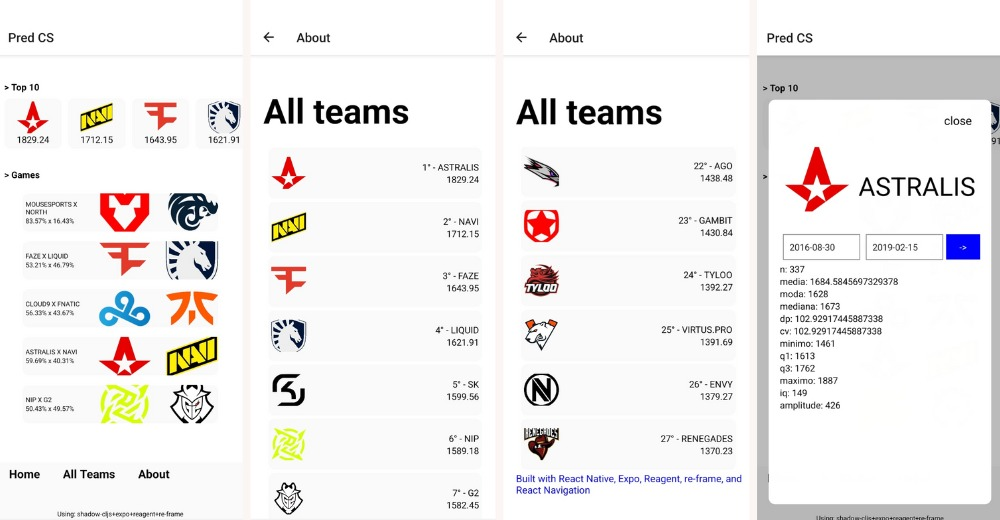
\includegraphics[width=16cm]{pred_cs_final.png}
\end{center}

O diagrama abaixo representa um fluxo de dados em um sistema que utiliza uma interface móvel (app) conectada a um backend via API REST, com funcionalidades de manipulação de dados, estado e lógica.

\begin{center}
  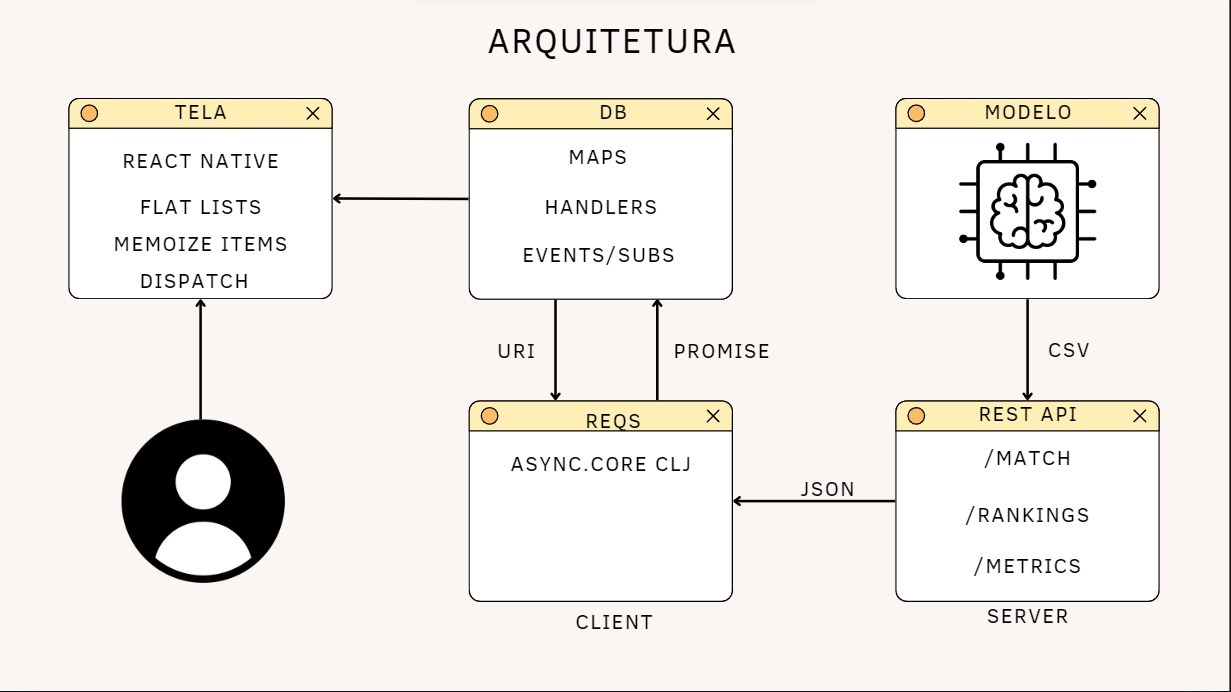
\includegraphics[width=12cm]{arquitetura.png}
\end{center}


\subsection{Destaques}
\hspace{+15pt}
Esta seção não contempla uma análise detalhadaa acerca do funcionamento das tecnologias que utlizou-se no projeto, entretanto, visa identificar as escolhas e o funcionamento geral do projeto. 

\subsubsection{Tela (Interface do Usuário):}
\begin{itemize}
  \item \textbf{Flat Lists:} Uma estrutura usada para exibir listas de dados de forma eficiente (por exemplo, uma lista de partidas esportivas).
  \item \textbf{Memoize Items:} Técnica para otimizar o desempenho, reutilizando itens já calculados ou renderizados.
  \item \textbf{Dispatch:} O envio de eventos (ações) que pedem mudanças no estado global da aplicação.
\end{itemize}
\noindent
\(\Rightarrow\) \textit{A Tela recebe os dados do banco de estado (DB) e envia eventos (ações) para modificar o sistema em paralelo a propria renderização.}

\subsubsection{DB (Banco de Estado):}
\begin{itemize}
  \item \textbf{Handlers:} Funções que processam eventos enviados pela tela (ex.: atualizar um placar).
  \item \textbf{Events/Subs:} Sistema de eventos (input) e assinaturas (output).
    \begin{itemize}
      \item \textit{Eventos:} Comandos que modificam o estado.
      \item \textit{Subscrições:} Consultas para acessar dados do estado.
    \end{itemize}
\end{itemize}
\noindent
\(\Rightarrow\) \textit{O DB é o coração da aplicação no lado do cliente, conectando a interface com o restante do sistema.}

\subsubsection{Requisições:}
\begin{itemize}
  \item \textbf{async.core:} Ferramentas em ClojureScript para lidar com chamadas assíncronas, como comunicação com a API.
  \item \textbf{Promise:} Uma estrutura para lidar com respostas de chamadas assíncronas (aguardando dados do servidor).
\end{itemize}
\noindent
\(\Rightarrow\) \textit{As REQS enviam e recebem dados da API REST, conectando o app com o servidor.}

\subsubsection{Modelo:}
\begin{itemize}
  \item Representa a lógica mais complexa do sistema.
  \item \textbf{CSV:} Arquivos usados para alimentar o modelo com dados brutos. Ademais, foram usasdos para transimitir os dados processados pelo modelo.
\end{itemize}
\noindent
\(\Rightarrow\) \textit{Ele alimenta o backend (API REST) com dados processados.}

\subsubsection{REST API (Servidor):}
\begin{itemize}
  \item Disponibiliza rotas como /match, /rankings e /metrics para fornecer ou receber informações.
  \item O backend processa dados e envia respostas em JSON para o cliente.
\end{itemize}
\noindent
\(\Rightarrow\) \textit{É o intermediário entre o modelo (dados e lógica) e o aplicativo no cliente.}

\subsection{Fluxo de Dados}
\begin{enumerate}
  \item O usuário interage com a \textbf{Tela} (ex.: visualiza uma lista ou clica em um botão).
  \item Um evento é \textbf{\textit{dispatched}} para o \textbf{DB}, que processa a lógica necessária.
  \item Se for necessário buscar dados externos, uma \textbf{requisição} é feita para a \textbf{REST API}.
  \item A \textbf{API} consulta o \textbf{Modelo} e retorna uma resposta.
  \item A resposta é processada no \textbf{DB}, e a \textbf{Tela} é atualizada com os novos dados.
\end{enumerate}

\section{Conclusão}
\hspace{+15pt}
O projeto foi concluído com êxito. Utilizou-se o modelo \textbf{Random Forest} para realizar a análise dos dados e observou-se uma satisfatória acurácia de 69\%. Dessa forma, o objetivo previamente estabelecido foi alcançado, uma vez que, com esta margem de acerto, a gama de testes, a aplicação e o servidor funcionais, pode-se garantir uma clara vantagem ao usuário em relação a predição de vencedores de partidas de Counter Strike. 


%%%%%%%%%%%%%%%%%%%%%%%%%%%%%%%%%%%%%%%%%%%%%%%%%%%%%%%%%%%%%%%%%%%%%%%%%%%%%
%%%%%%%%%%%%%%%%%%%%%%%%%%%%%%%%%%%%%%%%%%%%%%%%%%%%%%%%%%%%%%%%%%%%%%%%%%%%%
\newpage
\begin{thebibliography}{00}

  \bibitem{Predicting cs outcome} CHALMERS. Predicting the outcome of CS games using machine learning. 2018. Disponível em: https://publications.lib.chalmers.se/records/fulltext/256129/256129.pdf. Acesso em: [01 out. 2024].

  \bibitem{Predicting cs matches} LUND UNIVERSITY. Predicting Counter-Strike Matches. 2024. Disponível em: https://lup.lub.lu.se/luur/download?func=downloadFile\&recordOId=9145457. Acesso em: [02 out. 2024].

  \bibitem{HLTV} HLTV.org: your source for esports information. Disponível em: https://www.hltv.org. Acesso em: [29 set. 2024].

  \bibitem{cs-2} SVEC, O. Predicting Counter-Strike Game Outcomes with Machine Learning. Disponível em: https://dspace.cvut.cz/bitstream/handle/10467/99181/F3-BP-2022-Svec-Ondrej-predicting\_csgo\_outcomes\_with\_machine\_learning.pdf. Acesso em: [02 out. 2024].

  \bibitem{Kaggle} https://www.kaggle.com/datasets/gabrieltardochi/counter-strike-global-offensive-matches. Acesso em: [20 nov.2024].
\end{thebibliography}
\end{document}
